\section{Scoring \& Evaluation}

\subsection{Image Difference}

If you're handling simple binary images, you can perform a pixel difference comparison which just takes the first image XOR'd with the second, $I_1(x, y) \oplus I_2(x, y)$. The result (shown in Figure \cref{fig:crotchet-diff}) is a simple highlighting of the difference between the two.

\begin{figure}[h!]
  \centering
  
\includegraphics[width=\linewidth]{gfx/crochet-all.png}
  \caption{Highlighting differences between a perfect and a hand-drawn crochet}
  \label{fig:crotchet-diff}
\end{figure}

I really liked the simplicity of this approach and as a visual representation of perhaps `going outside the lines' it really gets the point across. However with some preliminary experiments it quickly became clear that it's not very useful in the context of scoring components like the crotchet in \cref{fig:crotchet-diff} where you can see by simple inspection that a small discrepancy in the scale of the note head contributes a much greater difference than a fairly significant error in the stem. If we therefore use the pixel difference outright we can't reasonably compare one component to another with respect to how `correct' it is.

\subsection{Normalized Cross Correlation}

Normalized cross correlation enables a pixel-wise comparison of two images, resulting in a score between $[-1, 1]$ where 1 indicates a perfect match \eg the images are the same and $-1$ indicates the images are precisely the opposite of each other. The overall effect is to penalise the score for each pixel which is different in one image than the other. The normalisation is designed to help in images where the brightness and light levels vary but it works fine on binary images too.

An NCC score between two binary images $F$ and $G$ of the same dimension can be calculated by using \cref{eqn:ncc}.

\begin{lequation}\label{eqn:ncc}
  \frac{1}{N} \sum_{x,y} \frac{\left( f(x,y) - \bar{f}\right)\left( g(x,y) - \bar{g}\right)}{\sigma_{f} \sigma_{g}}
\end{lequation}

Where $N = w \times h$ (the number of pixels in the image), $f(x,y)$ and $g(x, y)$ represent the pixel in row y column x for the respective images, $\bar{f}, \bar{g}$ represent the average pixel values for each image and $\sigma_{f},  \sigma_{g}$ are the standard deviations of the two images. 

\subsection{Skeletonization}
\label{sec:skeletonization}

Skeletonization is the process of reducing a component in a binary image to a single-pixel wide skeleton. The algorithm used in this project (as defined in \cite{zhang1984fast}) works by making successive passes of the image, removing pixels on object borders. This continues until no more pixels can be removed as in \cref{fig:skeletonization-example}.  The image is correlated with a mask that assigns each pixel a number in the range $[0...255]$ corresponding to each possible pattern of its $8$ neighbouring pixels. A look up table is then used to assign the pixels a value of $0, 1, 2$ or $3$, which are selectively removed during the iterations.

\begin{figure}[H]
  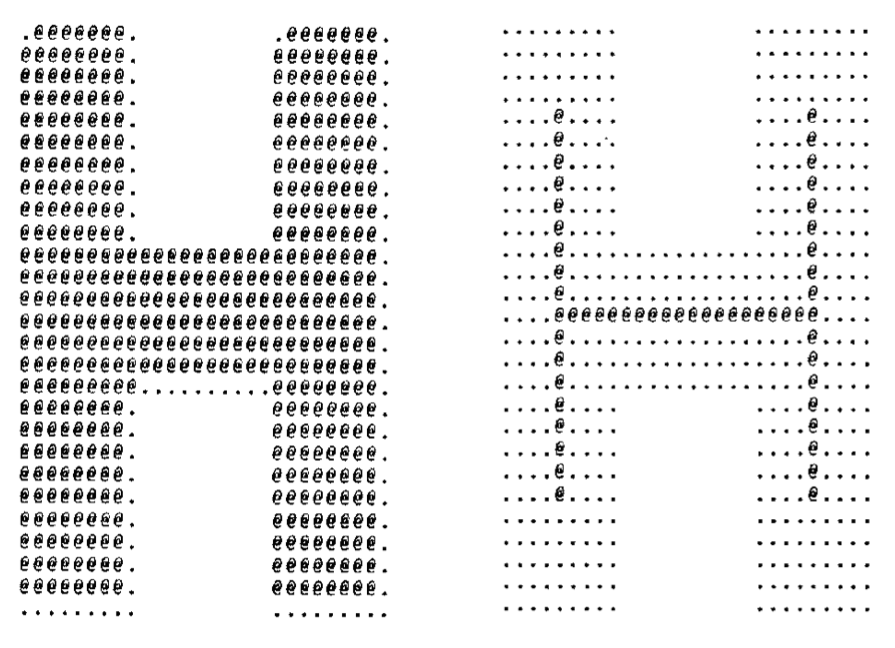
\includegraphics{gfx/skeletonization.png}
  \caption{Results of the skeletonization algorithm from \cite{zhang1984fast}}
  \label{fig:skeletonization-example}
\end{figure}


\subsection{Watershed Segmentation}

Watershed segmentation essentially allows us to segment an image by identifying starting points or `markers' from which we grow segments, marking the boundaries where these segments meet. There are multiple ways to add more pixels to the markers, one is to flood fill outwards from the marker. Another way which I found success in the context of the \noteED project is to perform a distance transform on the (binary) image, where pixels are assigned values according to how far they are from the nearest background pixel and use local maxima and assign pixels to the maxima depending on which marker is reachable by the steepest gradient ascent.

A good example from \citeauthor{scikit-watershed} is that of two overlapping circles we want to separate, shown in \cref{fig:watershed-circles}. The first step shows the two overlapping circles, the second shows a map of the distance transform. Here the dark red indicates a background pixel and the gradient ends with blue indicating the maximum distance from a background pixel. Local maxima are marked as starting points for the watershed algorithm. If we imagine the gradients as a 3D topographical map, and if we then assign pixels based on the steepest gradient ascent near them, they will group around the local maxima. Pixels which are equidistant from either peak result in a boundary forming which approximates the division between the original entities. We can now draw contours along these boundary lines to visually segment the image.

An example of watershed being used in \noteED to help find the centre of a broken flat is given in \cref{fig:flats-centre-watershed}.

\begin{figure}[hbt]
  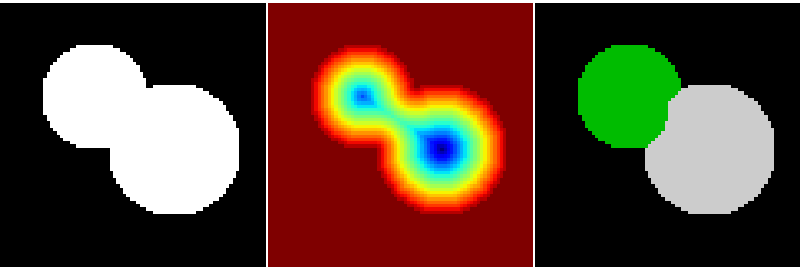
\includegraphics[width=\linewidth]{gfx/techniques/plot_watershed_1.png}
  \caption{Separating two overlapping circles using watershed segmentation from \citeauthor{scikit-watershed}}
  \label{fig:watershed-circles}
\end{figure}


